\chapter{Experiments and Results}
\label{chap:results}

\chapterguide{I evaluated component behaviour separately from complete task
execution because the two answer different questions. The evidence covers
software, language, perception, faults and closed-loop operation before being
mapped to objectives O1--O4.}

\contributionboundary
  {The starting repository contained no Room~315 evaluation protocols, campaign
  runners or evidence archive.}
  {The supervisors supplied scientific direction, platform knowledge and
  review; project resources supplied platform access, GPU time and simulation
  time.}
  {The evaluated system uses external ROS~2, Gazebo, Qwen2.5-1.5B, PlanSys2 and
  POPF. I implemented the tests with \code{pytest} \citep{pytest}; I built the
  vision pipeline with PyTorch \citep{pytorch} and TorchVision's ResNet-18
  \citep{torchvisionresnet18,resnet}. I developed none of these tools or base
  models.}
  {I designed and implemented the test suites, acceptance criteria, case
  matrices, runners, metrics, gates, provenance checks and evidence archive.}
  {I ran and reviewed every software, language, vision, observation, fault and
  closed-loop evaluation reported here. After qualification was frozen, I
  manually approved the Validation-selected V4 checkpoint for runtime; the
  Final Test did not alter the checkpoint, calibration or thresholds.}

\section{Closed-loop campaign result}
\label{sec:v4-closed-loop-campaign}

\subsection{Method and acceptance criteria}

Before execution, I fixed twelve case IDs, English instructions, expected
grounded goals and initial shuttle configurations. Slot goals named one
destination; station goals accepted any admissible slot. The runner bound the
source, language setup, epoch-11 visual checkpoint, runtime manifests and PDDL
domain by hash. It checked source/install parity and started every case in a
fresh Gazebo process and ROS Domain ID. Before accepting input, it awaited the
world, controllers, cameras, authorised perception, planner, supervisor and
gateway.

For each row, I checked the displayed interpretation and entered interactive
\code{yes}. Confirmation was never automated. Initial and final observations
had to use the declared schema and checkpoint. They also had to identify every
present shuttle's side, segment and payload correctly and keep
$|\Delta s_{ratio}|\leq0.12$ against the expected scene. A run passed only when
the requested terminal state, symbolic postconditions, DZI arrival evidence and
stopped-controller state agreed, with clean camera and ROS-bag closure. Case-level
paths and outcomes are summarised in \cref{app:technical}; full declarations and
retained records are indexed through \cref{app:reproducibility}.

\begin{table}[htbp]
\centering
\small
\caption{Coverage and outcome of the twelve-case closed-loop campaign.}
\label{tab:campaign-case-results}
\begin{tabularx}{\textwidth}{@{}p{0.22\textwidth}p{0.12\textwidth}Xp{0.13\textwidth}@{}}
\toprule
\textbf{Case group} & \textbf{Cases} & \textbf{Coverage} & \textbf{Result}\\
\midrule
Direct transfers & B01--B08 & Both rails, all eight shuttle identities, colour
aliases, explicit identities and station goals & 8/8 passed\\
\tablerowrule
Payload selection & P01--P02 & Loaded-nearest selection plus blocker clearance
on each rail & 2/2 passed\\
\tablerowrule
Multi-shuttle routes & M01--M02 & Four-step clearance and transfer route on
each rail & 2/2 passed\\
\bottomrule
\end{tabularx}
\end{table}

All 12 runs succeeded, all 24 step postconditions were satisfied and the
supervisor accepted the resulting 48 low-level proposals. The executive made
24 planner requests and replanned four times after occupancy changes; no run
needed an unknown-result retry or safe abort. Every run ended with
\code{task\_goal\_satisfied}, verified final effects and disabled controllers.
The 1,784 schema-compliant observations are recorded ROS messages, not
independent accuracy trials. Each scene was executed once, so the result proves
the declared Gazebo paths rather than repeated-run reliability.

\Cref{fig:b03-camera-evidence} gives a representative before/after comparison;
the corresponding DZI and controller records establish the terminal state.

\begin{figure}[htbp]
  \centering
  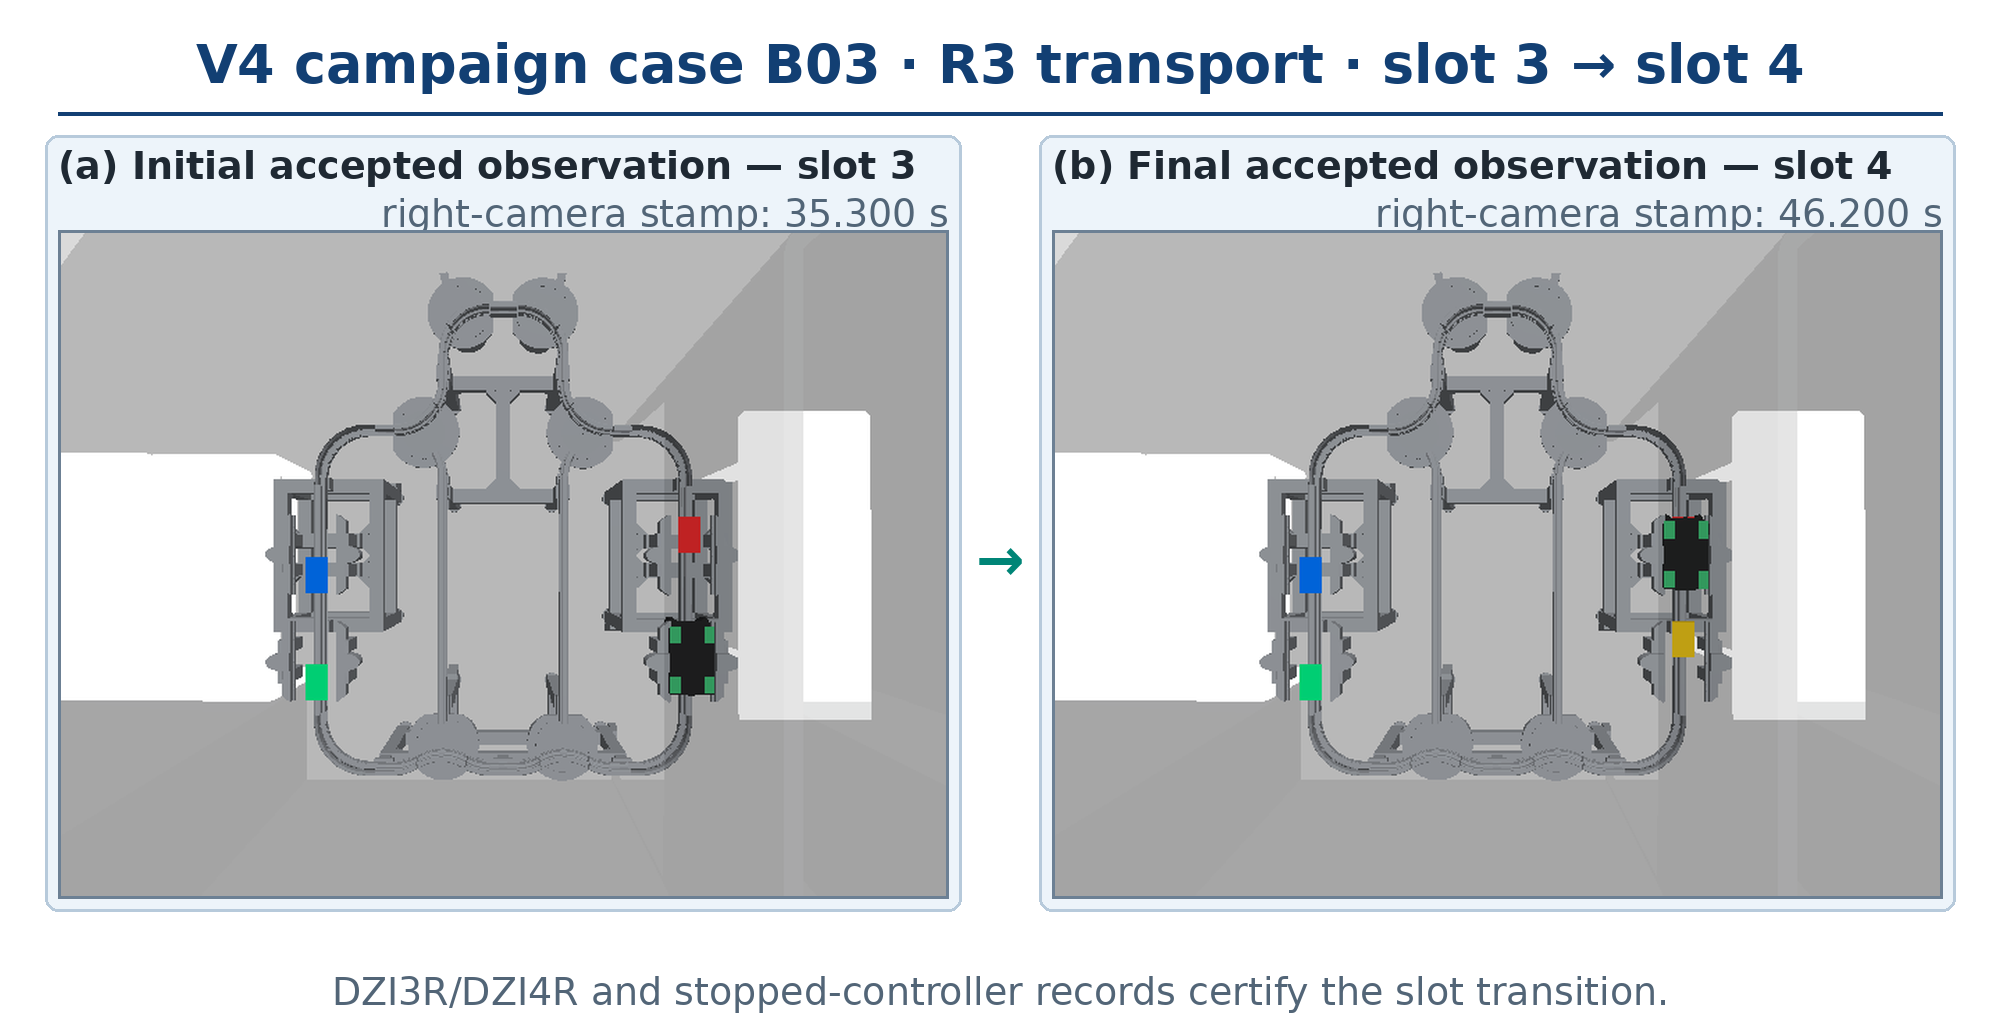
\includegraphics[width=0.99\textwidth]{images/b03_v4_closed_loop_right_camera_initial_final.png}
  \caption[Initial and final checkpoint-bound right-camera frames for case B03.]
  {Frames selected by the initial and final accepted observations in the B03
  ROS bag. Identity-bearing DZI3R/DZI4R and controller records establish R3's
  arrival at slot~4 and the final \code{DISABLED} controller state.}
  \label{fig:b03-camera-evidence}
\end{figure}

\FloatBarrier

\section{Final Test and runtime qualification}
\label{sec:visual-v4-results}

The Final Test evaluates the learned outputs in
\cref{fig:visual-model-contract}; topology-derived side, segment length and
metric position are excluded. Validation is the 512-scene selection set, while
the earlier 30 July Test is consumed and is not the Final Test below.

\subsection{One-shot Final Test method}

Frozen epoch~11 ran once on 1,040 scenes, 2,080 images and 4,680 visible
targets. Coverage selection used preregistered identifiers and aggregate support
counts only; no model predictions or individual image or label contents were
inspected. No training, model selection or calibration refit followed. The
protocol checked disjoint scene IDs,
generation-payload fingerprints, image bytes and complete label rows. It passed
76 preregistered model/support gates and four runtime-threshold gates. A gate is
one predeclared Boolean acceptance check, not an independent trial. The 76 gates
covered global, rail, segment, target-zone, position-bin, scene-stratum and
camera-counterfactual criteria. The four runtime gates covered minimum
segment-confidence coverage, loaded-state coverage, joint-confidence coverage
and selective segment accuracy. The checkpoint, sealed dataset, controls and
complete gate and stratum records are indexed through
\cref{app:reproducibility}; per-rail summaries are retained in
\cref{app:technical}.

Online checks decide whether an unlabelled prediction may enter the runtime;
offline labelled tolerances measure its error afterwards. With estimate
$\hat{s}_{ratio}$ and label $s^{\mathrm{label}}_{ratio}$, the reported error is
$|\Delta s_{ratio}|=|\hat{s}_{ratio}-s^{\mathrm{label}}_{ratio}|$. The distinct
uses are summarised in \cref{tab:visual-threshold-map}.

\begin{table}[htbp]
\centering
\small
\setlength{\tabcolsep}{5pt}
\renewcommand{\arraystretch}{1.05}
\caption{Online runtime checks and offline labelled tolerances.}
\label{tab:visual-threshold-map}
\begin{tabularx}{\textwidth}{@{}
>{\raggedright\arraybackslash}p{0.34\textwidth}X@{}}
\toprule
\textbf{Check} & \textbf{Interpretation}\\
\midrule
\multicolumn{2}{@{}l}{\textbf{Online runtime checks}}\\
Segment score $\geq0.9139$ & Temperature-scaled maximum over 14 segments. Below
the threshold, the whole paired observation is withheld; passing does not
guarantee correctness.\\
\tablerowrule
Loaded-state score $\geq0.5$ & Uncalibrated binary maximum. Because this maximum
is always at least 0.5, the check is non-selective; 0.5 does not mean 50\%
correctness.\\
\tablerowrule
$d_{\mathrm{slot}}=|\hat{s}_{ratio}-s^{\mathrm{slot}}_{ratio}|\leq0.12$ &
Distance to the configured slot anchor, used for occupancy. It is neither
confidence nor comparison with a hidden label.\\
\tablerowrule
\multicolumn{2}{@{}l}{\textbf{Offline labelled tolerances}}\\
Correct segment and $|\Delta s_{ratio}|\leq0.05$ & Strict ground-truth
diagnostic: error within 5\% of segment length, not \SI{5}{cm}.\\
\tablerowrule
Correct segment and $|\Delta s_{ratio}|\leq0.12$ & Planning/campaign-checker
tolerance for the expected scene: error within 12\% of segment length, not
\SI{12}{cm}. Although both use 0.12, this is not the online slot check.\\
\bottomrule
\end{tabularx}
\end{table}

Final arrival uses neither offline position tolerance: it requires
command-linked DZI and controller-state evidence as described in
\cref{chap:interfaces}.

Here, top-1 accuracy counts a target when the highest-scoring segment is its
labelled segment.

\begin{table}[htbp]
\centering
\small
\setlength{\tabcolsep}{4pt}
\caption{Global essentials from the one-shot Final Test.}
\label{tab:visual-v4-final-test-results}
\begin{tabularx}{\textwidth}{@{}X>{\centering\arraybackslash}p{0.23\textwidth}@{}}
\toprule
\textbf{Metric} & \textbf{Global result}\\
\midrule
Public-segment top-1 accuracy & 99.9359\%\\
\tablerowrule
Loaded-state accuracy & 99.9145\%\\
\tablerowrule
Joint segment and $|\Delta s_{ratio}|\leq0.05$ & 90.8974\%\\
\tablerowrule
Joint segment and $|\Delta s_{ratio}|\leq0.12$ & 99.0385\%\\
\tablerowrule
Correct-segment longitudinal mean absolute error (MAE) / 95th percentile &
\SI{0.01573}{m} / \SI{0.05850}{m}\\
\tablerowrule
Mean bounding-box intersection over union (IoU) & 0.83400\\
\bottomrule
\end{tabularx}
\end{table}

\FloatBarrier

V4 almost always recovered the discrete segment and loaded state needed by the
planner. Fine longitudinal localisation was weaker: 90.8974\% met the strict
0.05 diagnostic, whereas 99.0385\% met the 2.4-times wider planning tolerance.
The worst segment-recognition cell was left--A14 (94.6429\% recall on 56
targets); the weakest strict-position cell was left--A1E (61.9469\% at 0.05,
but 98.2301\% at 0.12 on 113 targets). Detailed per-rail, stratum and support
results remain in the Final-Test records indexed through
\cref{app:reproducibility}; the per-rail summary is in \cref{app:technical}.
These fixed-camera results do not establish physical-camera, unseen-condition or
complete task performance.

At the online segment floor, 4,678/4,680 targets were retained: two abstained,
while two different incorrect segment predictions passed. The loaded-state
floor retained all targets, including four incorrect decisions. Confidence
therefore controls acceptance rather than truth. Blanking or shuffling the
opposite camera changed own-side outputs by zero at recorded precision, whereas
swapping camera order reduced segment accuracy to 7.7991\%; this supports rail
isolation and the enforced camera order.

\subsection{Development and observation checks}

Validation passed 76/76 gates and selected the checkpoint and segment-score
calibration; the small post-selection regression set passed 74/74 gates and
could only reject the frozen candidate. Neither is independent evidence, so the
one-shot Final Test remains the reported evaluation. Full development metrics
are indexed through \cref{app:reproducibility}; \cref{app:technical} retains a
compact summary.

Observation-only checks disabled PlanSys2 mutation and actuation. Seven scenes
completed 53/53 reobservations at the 0.12 planning tolerance; 150/169 identity
checks also met the stricter 0.05 diagnostic. All eight injected visual-input
faults were rejected, and a dense-scene dry run produced 10/10 matching
reobservations. The isolated same-frame shadow accepted 52/55 pairs without
wrong-side identities or reported errors; the aggregate record does not explain
the remaining three rejections. Consequently, this result supports the
observation boundary but not motion or physical-camera performance.

\subsection{Closed-loop fault qualification}

Five faults were injected in fresh Gazebo processes. The case matrix in
\cref{tab:closed-loop-faults} makes the negative oracle explicit: the expected
result is a safe refusal or stop, never task completion.

\begin{table}[htbp]
\centering
\footnotesize
\renewcommand{\arraystretch}{0.96}
\caption{Closed-loop fault cases, expected response and recorded outcome.}
\label{tab:closed-loop-faults}
\begin{tabularx}{\textwidth}{@{}
>{\raggedright\arraybackslash}p{0.08\textwidth}
>{\raggedright\arraybackslash}p{0.25\textwidth}
>{\raggedright\arraybackslash}p{0.31\textwidth}
>{\raggedright\arraybackslash}X@{}}
\toprule
\textbf{Case} & \textbf{Injected fault} & \textbf{Predeclared safe response} &
\textbf{Recorded outcome}\\
\midrule
F01 & Corrupt authorisation & Reject before motion; no success record & Passed;
no false completion, controllers \mbox{\code{DISABLED}}\\ \tablerowrule
F02 & Invalid runtime manifest & Refuse runtime readiness and motion & Passed;
no false completion, controllers \mbox{\code{DISABLED}}\\ \tablerowrule
F03 & Missing planner service & End safely without publishing a motion command &
Passed; no false completion, controllers \mbox{\code{DISABLED}}\\ \tablerowrule
F04 & Emergency stop during a long move & Invoke \code{stop\_all}, latch the stop
and withhold completion & Passed; no false completion, controllers
\mbox{\code{DISABLED}}\\ \tablerowrule
F05 & Loss of right-sensor feedback & Do not certify arrival; stop or abort safely
& Passed; no false completion, controllers \mbox{\code{DISABLED}}\\
\bottomrule
\end{tabularx}
\end{table}

Across the five cases, all 5/5 criteria passed and all 424 observations used the
active schema. A subsequent B01 smoke run completed its step and postcondition
with 88 matching observations. Together, these records satisfy the declared
fault-response criteria.

\FloatBarrier

\section{Software, language and full-floor checks}
\label{sec:automated-evidence}

Three named suites checked the implementation before the integrated runs. The
contract/executive suite passed 190/190 checks, the transport suite 96/96 and
the complementary operator-capability suite 42/42. They cover geometry,
topology, identity, devices, reservations, language contracts, planning,
supervision and effect checks, with protective and fault cases. Because a few
files overlap, the suite counts are reported separately rather than summed;
their commands and logs are indexed in \cref{app:reproducibility}.

\subsection{Language-interface evaluation}
\label{sec:language-contract-evidence}

The fixed ten-case English corpus contained four supported goals, three
incomplete or ambiguous requests, two inconsistent or invalid requests and one
cancellation. All 10/10 final outcomes matched: valid goals produced the
expected constraints, uncertain requests requested clarification, invalid
requests were rejected and cancellation produced no task. The configured local
backend was called once for each of the nine non-control cases; eight envelopes
passed the strict schema, while the predicted invalid slot~9 was rejected. This
tests the implemented Room~315 contract, not open-vocabulary or multilingual
language understanding.

\subsection{All-robot launch check}

An isolated \code{robots:=all} cold start contained all six configured models.
Each exposed namespaced joint command and feedback topics and produced a fresh
\code{JointState}; both TIAGo variants also exposed independent base-velocity
topics, with no declared error pattern before shutdown. This one check supports
launch composition and namespace separation, not simultaneous motion or
repeatability. The complete record and operator procedures are indexed in
\cref{app:reproducibility}.

\section{Review of the internship objectives}

\Cref{tab:objective-results} returns to O1--O4 and links each objective to its
principal evidence.

\begin{table}[H]
\centering
\small
\caption{Assessment of the four internship objectives.}
\label{tab:objective-results}
\begin{tabularx}{\textwidth}{@{}
>{\raggedright\arraybackslash}p{0.19\textwidth}
>{\raggedright\arraybackslash}X
>{\raggedright\arraybackslash}p{0.20\textwidth}@{}}
\toprule
\textbf{Objective} & \textbf{Main result} & \textbf{Evaluation}\\
\midrule
O1---simulation platform & Third-floor CAD and room furnishings designed by me
in Autodesk Inventor; supplied rail-cell and attributed robot assets integrated
into full-floor and Room~315 scenes; selectable launch profiles retained &
Static geometry/SDF checks and one six-robot cold-start launch and interface
check\\
\tablerowrule
O2---multi-shuttle transport & Calibrated Hermite rail geometry, explicit
switch-dependent topology, eight stable identities, typed devices, reservations,
headway checks and bounded blocker staging on both rails & 96/96 named transport
checks and route-clearance cases in the integrated campaign\\
\tablerowrule
O3---contracts and supervision & Versioned command, state and effect contracts;
freshness and consistency gates; supervisor rejection paths; command-linked
post-step effect checks & 190/190 focused checks plus positive and fault campaign
records\\
\tablerowrule
O4---neuro-symbolic workflow & Rail-isolated perception and checked execution
from English requests; frozen Validation-selected V4 manually approved for the
Gazebo runtime without Final-Test-driven tuning & 10/10 language cases,
1,040-scene one-shot Final Test, 12/12 positive and 5/5 fault runs plus
observation-only qualification\\
\bottomrule
\end{tabularx}
\end{table}

Because the evaluations measure different properties, their counts are reported
separately. Each objective is considered achieved only within the limits of the
corresponding tests. Thus the launch check supports configuration and feedback,
the Final Test supports synthetic-camera perception, and the closed-loop
campaign supports the twelve declared tasks. Repeated operation was not
evaluated.

Overall, the results support O1--O4. Fine shuttle localisation remains the
weakest result:
90.8974\% at the 0.05 tolerance versus 99.0385\% at 0.12, while three of the 55
shadow comparisons remain unexplained. The evidence remains Gazebo-only and
neither authorises physical deployment nor establishes machinery-safety
certification.
